% Author: Till Tantau
% Source: The PGF/TikZ manual
\documentclass[12pt]{standalone}

\usepackage{tikz}
\usetikzlibrary{mindmap,trees}
\usepackage{verbatim}

\tikzset{font=\large}

\begin{document}
	\pagestyle{empty}
	
	\begin{comment}
	:Title: Computer science mindmap
	:Tags: Manual, Mindmap
	
	Version 1.09 of PGF/TikZ added a library for drawing mindmaps. Here's an example
	from the manual. 
	
	| Author: Till Tantau
	| Source: The PGF/TikZ manual
	
	
	
	\end{comment}
	
	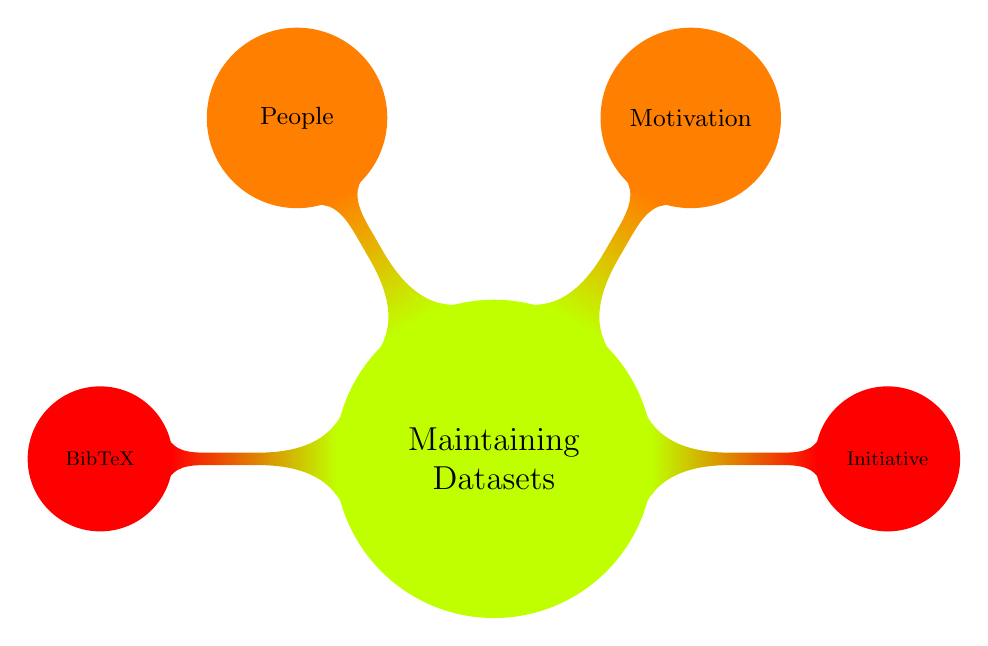
\begin{tikzpicture}
	\path[mindmap,concept color=lime, text=black]
		node[concept] {Maintaining Datasets}
		[clockwise from=180]
		child[concept color=red] { 
			node[concept, scale=0.8] {BibTeX} 
		}
		%[clockwise from=90]
		child[concept color=orange] { 
			node[concept] {People} 
		}
		child[concept color=orange] { 
			node[concept] {Motivation} 
		}
		child[concept color=red] { 
			node[concept, scale=0.8] {Initiative} 
		}
		;
		
	\end{tikzpicture}\end{document}